\section{电功}\label{sec:9-1}

我们已经知道电流可以做功。
例如,在图 \ref{fig:9-1} 所示的实验里,给小电动机通电,电动机将砝码提起,这时电流做了功。
在这个做功过程中,电能转化为机械能。

\begin{wrapfigure}{r}{7cm}
    \centering
    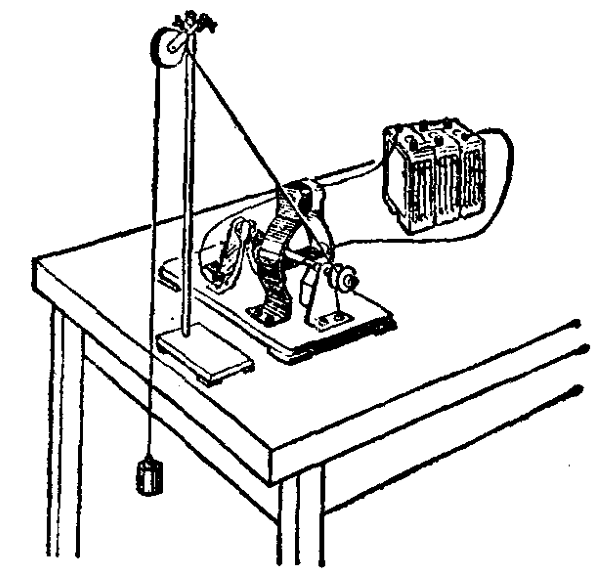
\includegraphics[width=6cm]{../pic/czwl2-ch9-1}
    \caption{}\label{fig:9-1}
\end{wrapfigure}

在电流通过电灯的做功过程中,电能转化为热能(其中部分热能又转化为光能)。
在电流给蓄电池充电的做功过程中,电能转化为化学能。

总之,电流做功的过程,实际就是电能转化为其他形式的能的过程。
电流做了多少功,就有多少电能转化为其他形式的能。

我们还知道,电流通过导体所做的功,跟导体两端的电压、通过导体的电量有关系。
怎样计算电流所做的功呢?

在 “\hyperref[sec:8-3]{电压}” 一节中学过,
如果电路两端的电压是 1  伏特,那么电路中每通过 1 库仑电量,电流做 1 焦耳的功。
如果电路两端的电压是 10 伏特,那么电路中每通过 1 库仑电量,电流就做 10 焦耳的功。
这就是说,电路两端电压的伏特数,等于每通过 1 库仑电量时电流做功的焦耳数。
如果通过的电量不是 1 库仑而是几库仑,电流做的功也就增加到几倍。
所以电流在某段电路上做的功 $W$(焦耳),等于这段电路两端的电压 $U$ (伏特)
与通过的电量 $Q$(库仑)的乘积,即 $W = UQ$。

电量 $Q$ 不容易直接测出,所以 $W = UQ$ 在实际工作中用起来不方便。
但是电量 $Q$ 等于电流强度 $I$ 与时间的乘积($Q = It$), 而 $I$、$t$ 是容易测出的。
因此,计算电功经常用的是下面的公式:
$$ W = UIt \;\juhao $$
上式表明,\textbf{电流在某段电路上所做的功,等于这段电路两端的电压与电路中的电流强度以及通电时间的乘积}。

如果式中 $U$ 的单位用伏特,$I$ 的单位用安培,$t$ 的单位用秒,那么 $W$ 的单位就是焦耳。

电功的位 “焦耳” 也就是机械功的单位 “焦耳”,即
$$ 1\jiaoer = 1\niudunmi = 1\text{伏特·安培·秒} = 1\text{伏特·库仑} \;\juhao $$

通过手电筒灯泡的电流,每秒钟做的功大约是 1 焦耳。
通过普通电灯泡的电流,每秒钟做的功一般是几十焦耳。


\liti 一盏电灯连在电压是 220 伏特的电路上,灯泡中的电流强度是 68 亳安,通电 1 小时,
电流做了多少焦耳的功?消耗了多少电能?

根据已知条件,可以用公式 $W = UIt$ 来计算电流做的功,
但是必须注意 $U$、$I$、$t$ 的单位分别用伏特、安培、秒,$W$ 的单位才是焦耳。

电流做了多少功就表示有多少电能转化为其他形式的能,
所以,求出电流做功的焦耳数,也就知道了消耗的电能值。

解:$\begin{aligned}[t]
    W &= UIt \\
      &= 220\fute \times 0.068\anpei \times 3600\miao \\
      &\approx 5.4 \times 10^4\jiaoer \;\juhao
\end{aligned}$

答: 电流做了 $5.4 \times 10^4$ 焦耳的功,消耗了 $5.4 \times 10^4$ 焦耳的电能。


\lianxi

(1) 一个电热器所用的电压是 220 伏特,电流强度是 0.23 安培,通电 5 分钟电流做了多少功?消耗的电能是多少?

(2) 将一小电动机接在电压为 12 伏特的电源上,在 10 分钟内电流做了 3600 焦耳的功。通过电动机的电流强度是多?

(3) 把一个工作时电阻是 80 欧姆的电炉,接在照明电路中,要它放出 26400 焦耳的能量,通电的时间应该是多少?

(4) 把一个电阻为 20 欧姆的导体,接在某一电源上。
在这个导体上每通过 3 库仑的电量,电流做 18 焦耳的功。
求电源的电压和导体中的电流强度。

(5) 并联在电路里的两盏电灯 $L_1$ 和 $L_2$,如果 $L_1$ 的电阻比 $L_2$ 的电阻大,
那么,通过哪盏灯的电流强度大?在相等时间里,电流通过哪盏灯所做的功多?哪盏灯更亮些?

(6) 串联在电路里的两盏电灯 $L_1$ 和 $L_2$,如果 $L_1$ 的电阻比 $L_2$ 的电阻大,
那么,哪盏灯两端的电压大?在相等时间里,电流通过哪盏灯所做的功多?哪盏灯更亮些?

